\documentclass{article}

\PassOptionsToPackage{numbers,compress}{natbib}
\usepackage[preprint]{neurips_2026}

\usepackage[utf8]{inputenc}
\usepackage[T1]{fontenc}
\usepackage{lmodern}
\usepackage{hyperref}
\usepackage{url}
\usepackage{booktabs}
\usepackage{array}
\usepackage{amsfonts}
\usepackage{amsmath}
\usepackage{amssymb}
\usepackage{microtype}
\usepackage{graphicx}
\usepackage[switch]{lineno}
\graphicspath{{../}}

\usepackage{caption}
\captionsetup{font=small,labelfont=bf,labelsep=period}

\title{Recognizing the predictive boundary of\\historically restricted physical knowledge}

\author{%
  Chenxi He\thanks{Correspondence: \texttt{ch2067@cam.ac.uk}} \\
  Cavendish Laboratory\\
  University of Cambridge\\
  Cambridge CB3 0HE, United Kingdom \\
  \And
  Jingqiu Chen \\
  College of Physics and Optoelectronic Engineering\\
  Shenzhen University\\
  Shenzhen 518060, China \\
}

\begin{document}
\maketitle
\linenumbers

\begin{abstract}
Scientific models have finite domains, normally established only in
hindsight, once a successor theory explains the failure. Machine-learning
systems for scientific data are optimized to interpolate, to predict forward, or
to recover a governing expression; none asks where an established description
ceases to hold. Here we show that the reach of a body of physical knowledge can
be recovered from that knowledge alone. We restrict a representation to
relations recorded before a chosen date, give it no later formula and no example
of a departure, and require it to rank measurements that knowledge cannot
account for. At an 1899 horizon, an encoder trained on source-audited pre-1900
point clouds ranks twentieth-century physical laws above held-out classical ones
with an area under the ROC curve of 0.925, against 0.649 before optimization; an
independently frozen extrapolation test reaches 0.888 with no learned
representation at all. A discrepancy found this way is tied to the incumbent
model rather than to the data: on historical measurements it collapses when, and
only when, the successful successor prediction is admitted. The same test can be
moved to any period for which a dated corpus exists.
\end{abstract}

\section{Introduction}

Physics advances by retiring descriptions that have stopped working. The
Rayleigh--Jeans law, the Dulong--Petit law and the classical account of
electrical resistance were each accurate across the range in which they were
built and each failed outside it, and in every case the failure was recognized
only once a successor theory had supplied the explanation. The domain over which
a model can be trusted is therefore something the field has established in
retrospect.

Machine-learning systems for scientific data are built for other targets. They
are optimized to interpolate within a sampled range, to predict forward, or to
recover a compact governing expression from
observations~\cite{wang2023discovery,xu2021extrapolate}. Conformal prediction
calibrates residuals, change-point methods locate distributional shifts, and
Bayesian model discrepancy compares observations with a
simulator~\cite{angelopoulos2023conformal,page1954cusum,kennedy2001bayesian}.
Symbolic regression searches for a replacement expression once a discrepancy has
already been found~\cite{guimera2020bayesian,udrescu2020feynman}.

None of these operations specifies which body of physical knowledge is under
test. A residual is large relative to some fitted model, a change point is a
shift in some distribution, and a recovered expression is a fit to some data; in
each case the knowledge being audited is implicit in the setup rather than
declared. Nor can shape novelty close the gap, because a physically decisive
departure may keep an entirely ordinary functional form while a familiar
mechanism may produce a highly unusual one.

Here we make the knowledge horizon an explicit input and test it directly with
EPOCH (Epistemic Probe of Classical Horizons). Every test declares its
admissible model set, fitted parameters, observation and censoring model,
fitting data, complete adaptive procedure, statistic and error rate, and returns
one of four verdicts: compatibility over the measured range, a localized
boundary with an uncertainty interval, incompatibility over the sampled range
with no identifiable boundary, or abstention. Three kinds of evidence are
reported separately rather than averaged into a single score: a positive-only
representation of the declared corpus, data-anchored extrapolation from a
sampled incumbent regime, and a theory-conditioned residual test against a
case-matched null.

We set the horizon at 1899, the eve of the largest replacement of a model set in
the history of physics and the last date at which the classical corpus can still
be reconstructed from dated primary sources. Every admitted training relation is
linked to a dated source-law family, splits are grouped by family, and the
learned optimization contains neither later formulas nor artificial breakdown
templates; the large-scale protocol was timestamp-frozen before any temporal
score was computed. We find that a representation built this way ranks
twentieth-century formula families above held-out pre-1900 groups, that explicit
extrapolation reaches the same conclusion without a learned representation, that
the discrepancy found on five historical datasets collapses only under the
successful successor prediction and not under wrong-shape or wrong-mechanism
alternatives, and that on real measured series the leading source of variation
is the observation process rather than the period of the underlying physics.

\section{Results}

\subsection{Declaring the object of a boundary test}

EPOCH returns one of four verdicts for a set of measurements and a declared
model set: compatible over the measured range; localized model incompatibility
with an uncertainty interval; model incompatibility over the sampled range with
no identifiable boundary; or insufficient evidence (Fig.~\ref{fig:concept}).
Which evidence produces the verdict is fixed in advance. Data-anchored evidence
is used when a clean incumbent interior is observed, theory-conditioned evidence
otherwise if an incumbent prediction and an uncertainty model are available, and
the test abstains when neither route is supported.

\begin{figure}[t]
  \centering
  \includegraphics[width=\textwidth,keepaspectratio]{figures/Figure_1_concept.png}
  \caption{\textbf{Testing a declared knowledge horizon.} Top, a system
  restricted to physics recorded before 1900 carries that corpus to the edge of
  what it predicts. An admitted classical form fitted inside the sampled regime
  (blue) tracks the measurements until they leave it; beyond that point the
  extrapolation and the data separate, and the question is whether the
  separation can be measured and located. Bottom, the test as applied here. A
  notation-free point cloud carrying no formula, unit or label enters at the
  left. A fixed rule identifies a contiguous interior regime and fits an admitted
  pre-1900 form there, the extrapolation is compared with the frontier through
  split-conformal nonconformity and an extrapolation-residual ratio, and a
  positive-only encoder trained on pre-1900 relations alone supplies an
  independent representation distance. The signpost carries the verdict and,
  where an incumbent regime is sampled, the location at which compatibility is
  lost; a fourth output, abstention, applies when neither evidence route is
  supported.}
  \label{fig:concept}
\end{figure}

The three components are calibrated against their own reference distributions
and reported separately rather than averaged. The data-anchored component
receives a notation-free point cloud, fits the best admissible generic form on a
contiguous interior regime and tests its extrapolation at the frontier through
split-conformal nonconformity and an extrapolation-residual ratio over power,
exponential, linear and constant fits. The theory-conditioned component forms
measurement-model-aware residuals against a named incumbent prediction and tests
them against a case-matched counterfactual null. The learned component measures
distance from a positive-only representation of relations recorded before the
declared date. Every test declares its admissible model set, fitted parameters,
observation and censoring model, fitting data, complete adaptive procedure,
discrepancy statistic and error rate, and a named physical-theory conclusion
follows only when the model set and observation model encode that theory's
relevant predictions (Methods). Table~\ref{tab:principal} collects the principal
quantitative results reported below.

\begin{table}[t]
\centering
\caption{\textbf{Principal quantitative results.}}
\label{tab:principal}
\small

\begin{tabular}{@{}>{\raggedright\arraybackslash}p{0.46\textwidth}
                  >{\raggedright\arraybackslash}p{0.46\textwidth}@{}}
\toprule
Analysis & Result \\
\midrule
Large learned model, 38 families from 1901--1950 vs nine pre-1900 groups &
AUROC 0.921 [0.833, 0.994]; unoptimized 0.589 \\
Large learned model, 55 families from 1901--1996 vs nine pre-1900 groups &
AUROC 0.925 [0.851, 0.982]; unoptimized 0.649 \\
Generator-matched learned analysis, 55 later vs nine pre-1900 groups &
AUROC 0.857 [0.741, 0.945]; unoptimized 0.545 \\
Independently frozen four-form analysis, 55 later vs 11 pre-1900 families &
AUROC 0.888 [0.800, 0.959] \\
Source-audited compact encoder vs matched generic-function encoder &
Family AUROC 0.903 [0.729, 1.000] vs 0.375 [0.167, 0.618] \\
Blinded transfer, 200 classical records and 30 synthetic departures &
AUROC 0.88 \\
Calibrated data-anchored decision, 12 departure and 12 classical families &
TPR 0.271 [0.073, 0.500]; 0/96 false positives at the 5\%-targeted threshold \\
Clock advancement on identical data grids &
4/5 old-horizon mismatches clear under the successful successor prediction \\
Horizon-specificity controls &
5/5 wrong-shape and 5/5 wrong-mechanism predictions remain rejected \\
Frozen components on sixteen measured series, 5 post-1900 vs 9 classical or
metrological groups &
Learned AUROC 0.62 [0.29, 0.89]; four-form AUROC 0.78 [0.38, 1.00] \\
Boundary localization on 900 held-out simulations &
90\% interval coverage 91.3\% [89.3\%, 93.0\%] \\
Observation-process stress test at maximum severity &
FPR 0.40 for saturation; 0.63 for censoring; $\leq 0.11$ for all other tested
effects \\
\bottomrule
\end{tabular}
\end{table}

\subsection{Recognizing later physics from pre-1900 relations alone}

To ask how much of a knowledge boundary is visible in the shape of a relation
alone, we trained a 20.9-million-parameter encoder on 880,896 normal-law point
clouds derived from 3,441 source-audited pre-1900 formula reductions. The model
aligns a permutation-invariant point-cloud student to a training-only
formula-graph teacher; at inference it receives an unordered normalized point
cloud and nothing else, with no formula, graph, units, date, source or anomaly
label. Data views, checkpoint rule, score construction, aggregation and
bootstrap procedure were timestamp-frozen before any temporal score was
computed.

Against nine held-out pre-1900 historical-family groups, the 1899-horizon score
separates 38 citation-anchored families dated 1901--1950 with AUROC
0.921 [0.833, 0.994], 17 post-1950 families with 0.935 [0.823, 1.000] and their
55-family union with 0.925 [0.851, 0.982] (Figs.~\ref{fig:transfer}a and
\ref{fig:learned}). The same-seed, architecture-matched model before
optimization reaches 0.589, 0.784 and 0.649. All four trained score components
separate the 55-family union on their own, with AUROCs from 0.800 to 0.925.

\begin{figure}[t]
  \centering
  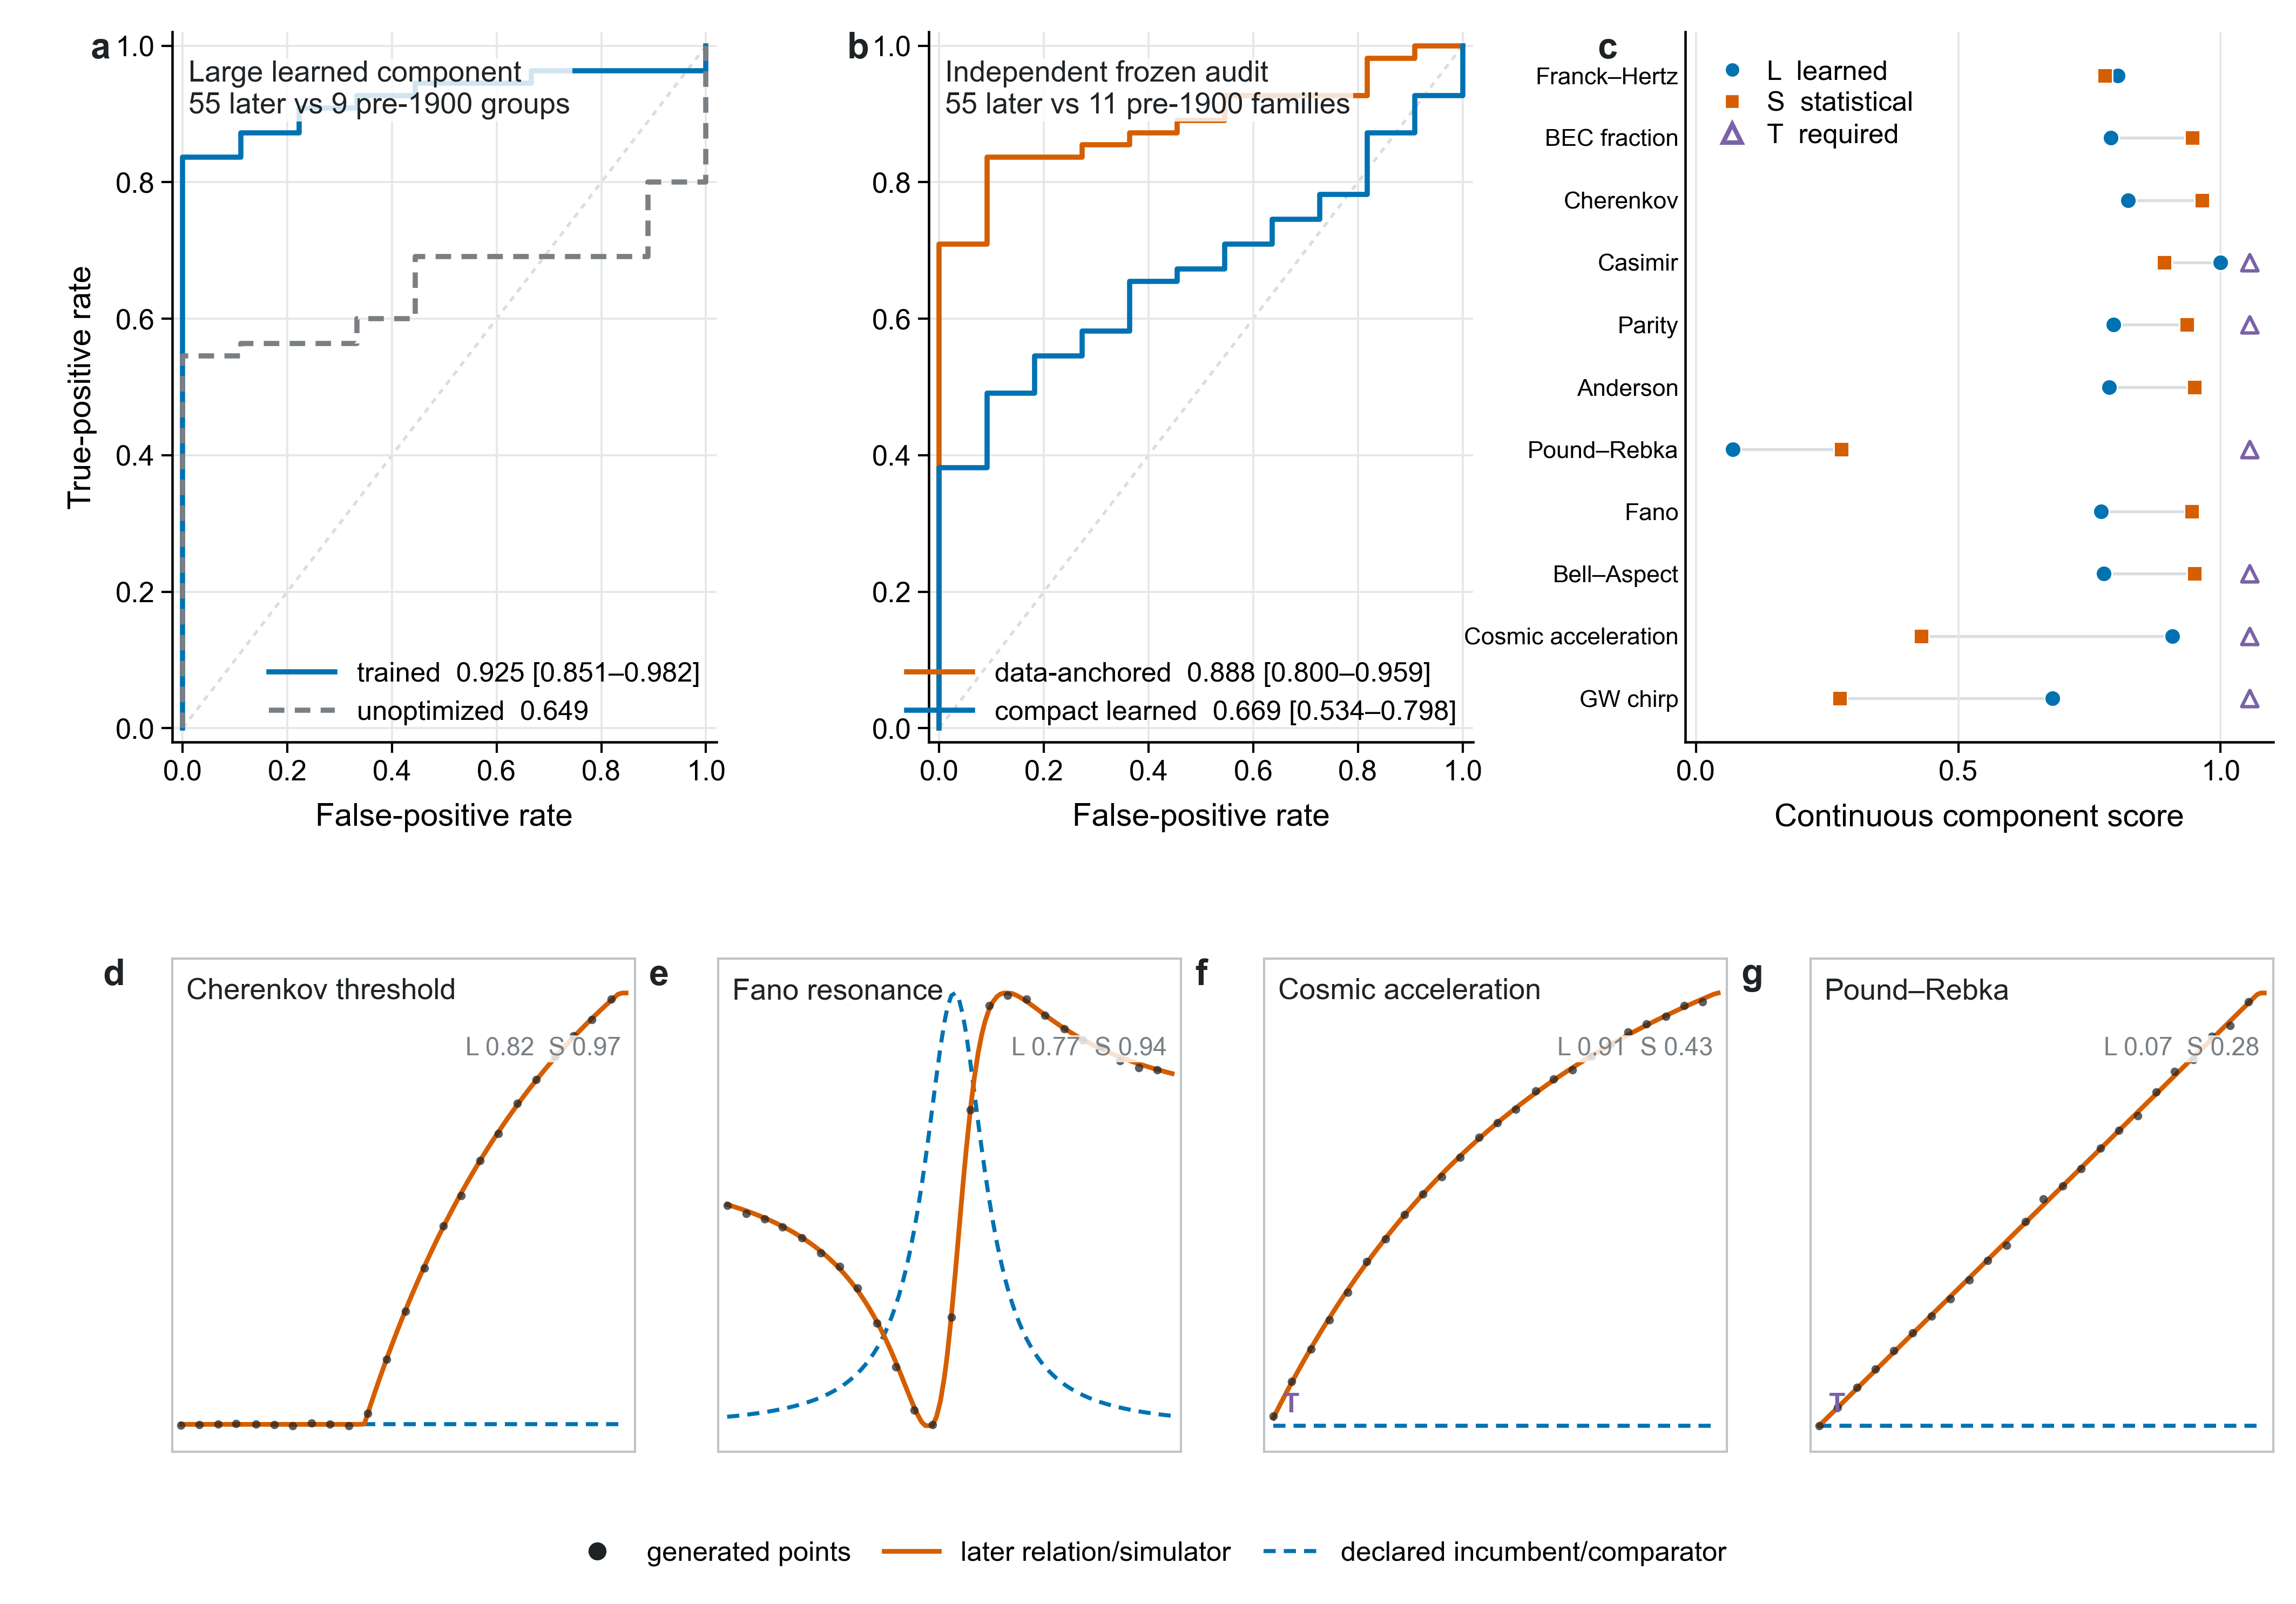
\includegraphics[width=\textwidth,keepaspectratio]{figures/figure_case_study_composite.png}
  \caption{\textbf{Temporal transfer and component scores across later physics.
  a}, ROC curves for the 20.9-million-parameter encoder trained on pre-1900 point
  clouds (blue) and the same architecture before optimization (grey), comparing
  55 later formula families with nine pre-1900 groups. \textbf{b}, Independent
  audit of the data-anchored component (orange) and compact learned encoder
  (blue) against 11 cited pre-1900 families. \textbf{c}, Learned scores
  (L, circles) and size-matched statistical percentiles (S, squares) for 11
  development cases. Triangles mark cases routed to an incumbent-conditioned test
  (T). \textbf{d--g}, Point clouds, later relations and incumbent comparators for
  Cherenkov emission~\cite{frank1937}, Fano resonance~\cite{fano1961}, cosmic acceleration~\cite{riess1998} and Pound--Rebka redshift~\cite{pound1960}. Checkpoints and calibration objects remain fixed throughout.}
  \label{fig:transfer}
\end{figure}

\begin{figure}[t]
  \centering
  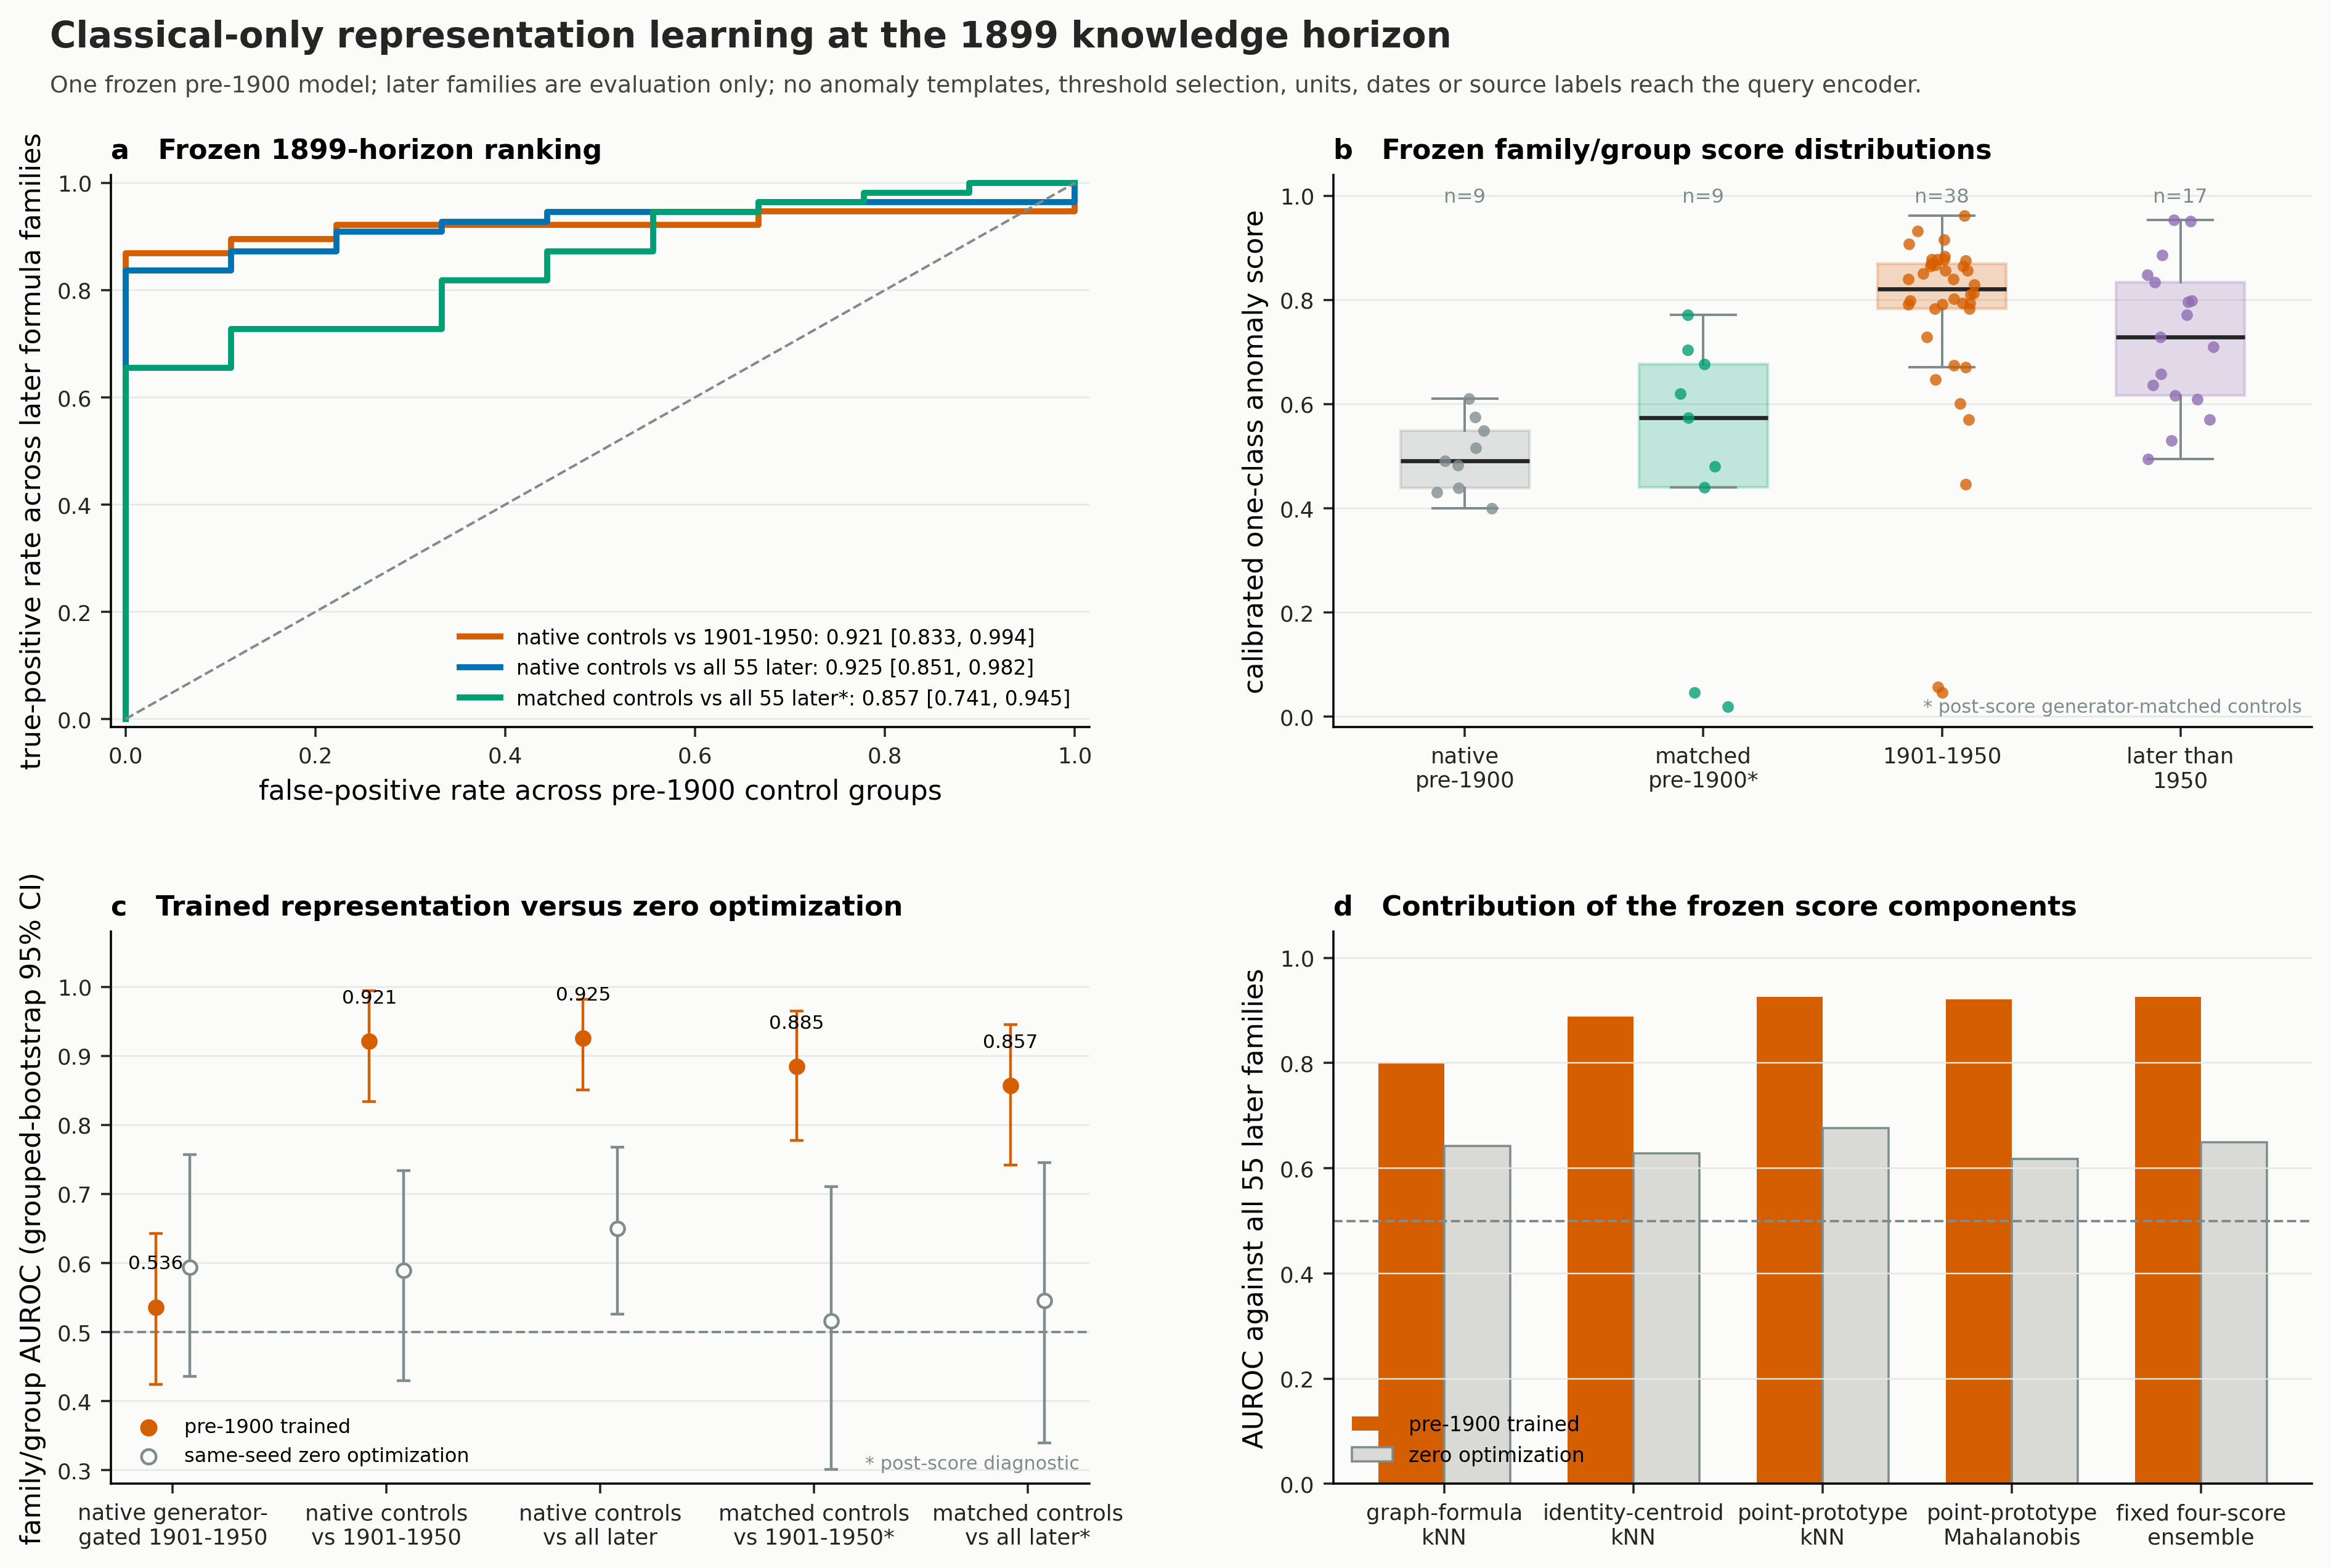
\includegraphics[width=\textwidth,keepaspectratio]{figures/figure_learned_pre1900_v3.png}
  \caption{\textbf{Large-scale representation audit at the 1899 horizon. a}, The
  frozen model separates 38 families dated 1901--1950 and all 55 later families
  from nine pre-1900 groups. All-later AUROC is 0.857 [0.741, 0.945] against
  generator-matched controls. \textbf{b}, One-class score distributions for
  native and matched pre-1900 controls and the two later-era strata. \textbf{c},
  AUROCs for trained and same-seed zero-optimization models. The native
  generator-gated comparison is shown separately. \textbf{d}, Each of the four
  distance components and their fixed equal-weight mean improves over zero
  optimization on the 55-family comparison. Inferential units are source-law
  families or frozen relation groups.}
  \label{fig:learned}
\end{figure}


Sampling alone could in principle produce that separation, because the later
families were generated by a different process from the internal pre-1900
corpus. Regenerating all nine internal groups under the later benchmark's point
count, x-jitter, repeat count, noise range and heteroscedastic profile leaves
AUROC at 0.885 [0.778, 0.965] for the 38 near-future families and
0.857 [0.741, 0.945] for all 55, against 0.516 and 0.545 before optimization.
Pre-1900 optimization therefore contributes beyond the generator contrast, with
the nine negative families governing the interval.

The gain is specific to the historical corpus rather than to function exposure
in general. A source-audited reconstruction supplies 268 point clouds from 51
cited pre-1900 law families, split by family into 205/17/46 training, validation
and test records, and a compact encoder trained on the 205 classical records
without deformation negatives reaches family AUROC 0.903 [0.729, 1.000], against
0.329 and 0.288 for matched random features under kNN and shrinkage Mahalanobis.
A capacity- and data-matched encoder trained instead on generic smooth
expressions, with identical architecture, seed, schedule, record count,
family-size profile and functional-signature histogram, reaches
0.375 [0.167, 0.618]; the paired difference is 0.528 [0.264, 0.764], and across
three paired seeds the two ranges are 0.889--0.910 and 0.292--0.403. A
unit-preserving deformation audit gives source-family-balanced AUROC 0.684 with
dimensional labels and 0.922 without them, so the zero-unit ranking is not
carried by units.

\subsection{Explicit extrapolation as independent evidence}

Explicit extrapolation reaches the same conclusion without a learned
representation. A citation-anchored audit contains 55 named physical-law
families first valid from 1901 to 1996, with eight independently sampled and
noisy 120-point realizations each, giving 440 formula-generated point clouds
(Fig.~\ref{fig:transfer}b); eleven cited pre-1900 families excluded from encoder
training serve as controls. Neither component is retrained or recalibrated here,
the zero-unit encoder, its pre-1900 reference bank and the four-form statistical
scorer being frozen beforehand, and all quantities are reduced to one median per
source-law family.

The four-form component ranks later families above the earlier holdouts with
AUROC 0.888 [0.800, 0.959], and the compact learned component with
0.669 [0.534, 0.798]. A blinded evaluation over 200 historical formula records
and 30 synthetic realizations of five breakdown families gives 0.88, with recall
0.90 and a false-positive rate of 0.24 at the 0.5 screening threshold.

Functional structure explains part of the ranking. Learned and statistical
AUROCs are 0.629/0.795 for 12 later affine, power or exponential laws,
0.600/0.982 for five threshold or piecewise families, and 0.909/0.864 for six
nonmonotone or oscillatory families, so the two scores respond differently to
smooth familiar forms, to thresholds and to nonmonotone curves.

Applied without retraining to 11 further twentieth-century cases
(Fig.~\ref{fig:transfer}c--g), the two coordinates diverge again: Casimir plates~\cite{casimir1948}
give 1.000/0.892, Cherenkov emission~\cite{frank1937} 0.823/0.965, cosmic acceleration~\cite{riess1998,perlmutter1999} 0.908/0.429 and Pound--Rebka redshift~\cite{pound1960} 0.071/0.277. Scalar or sparse-level
claims, including the Lamb shift~\cite{lamb1947} and the electron anomalous magnetic moment~\cite{schwinger1948},
route to the theory-conditioned component instead, and the primary AUROC is
unchanged (Supplementary Note~17).

\subsection{Historical measurements at the 1899 horizon}

Four historical datasets cover the two outputs available when the incumbent is a
named classical law: whole-range model rejection and boundary localization
(Fig.~\ref{fig:cases}a--d). The initial data-anchored screen gives percentiles of
0.95 for FIRAS, 0.95 for copper specific heat, 0.66 for Bertozzi and 0.66 for
Onnes; case-specific tests then determine which output the measurements support.
Supplementary Note~5 gives finite-sample tail probabilities and the multiplicity
calculation.

\begin{figure}[t]
  \centering
  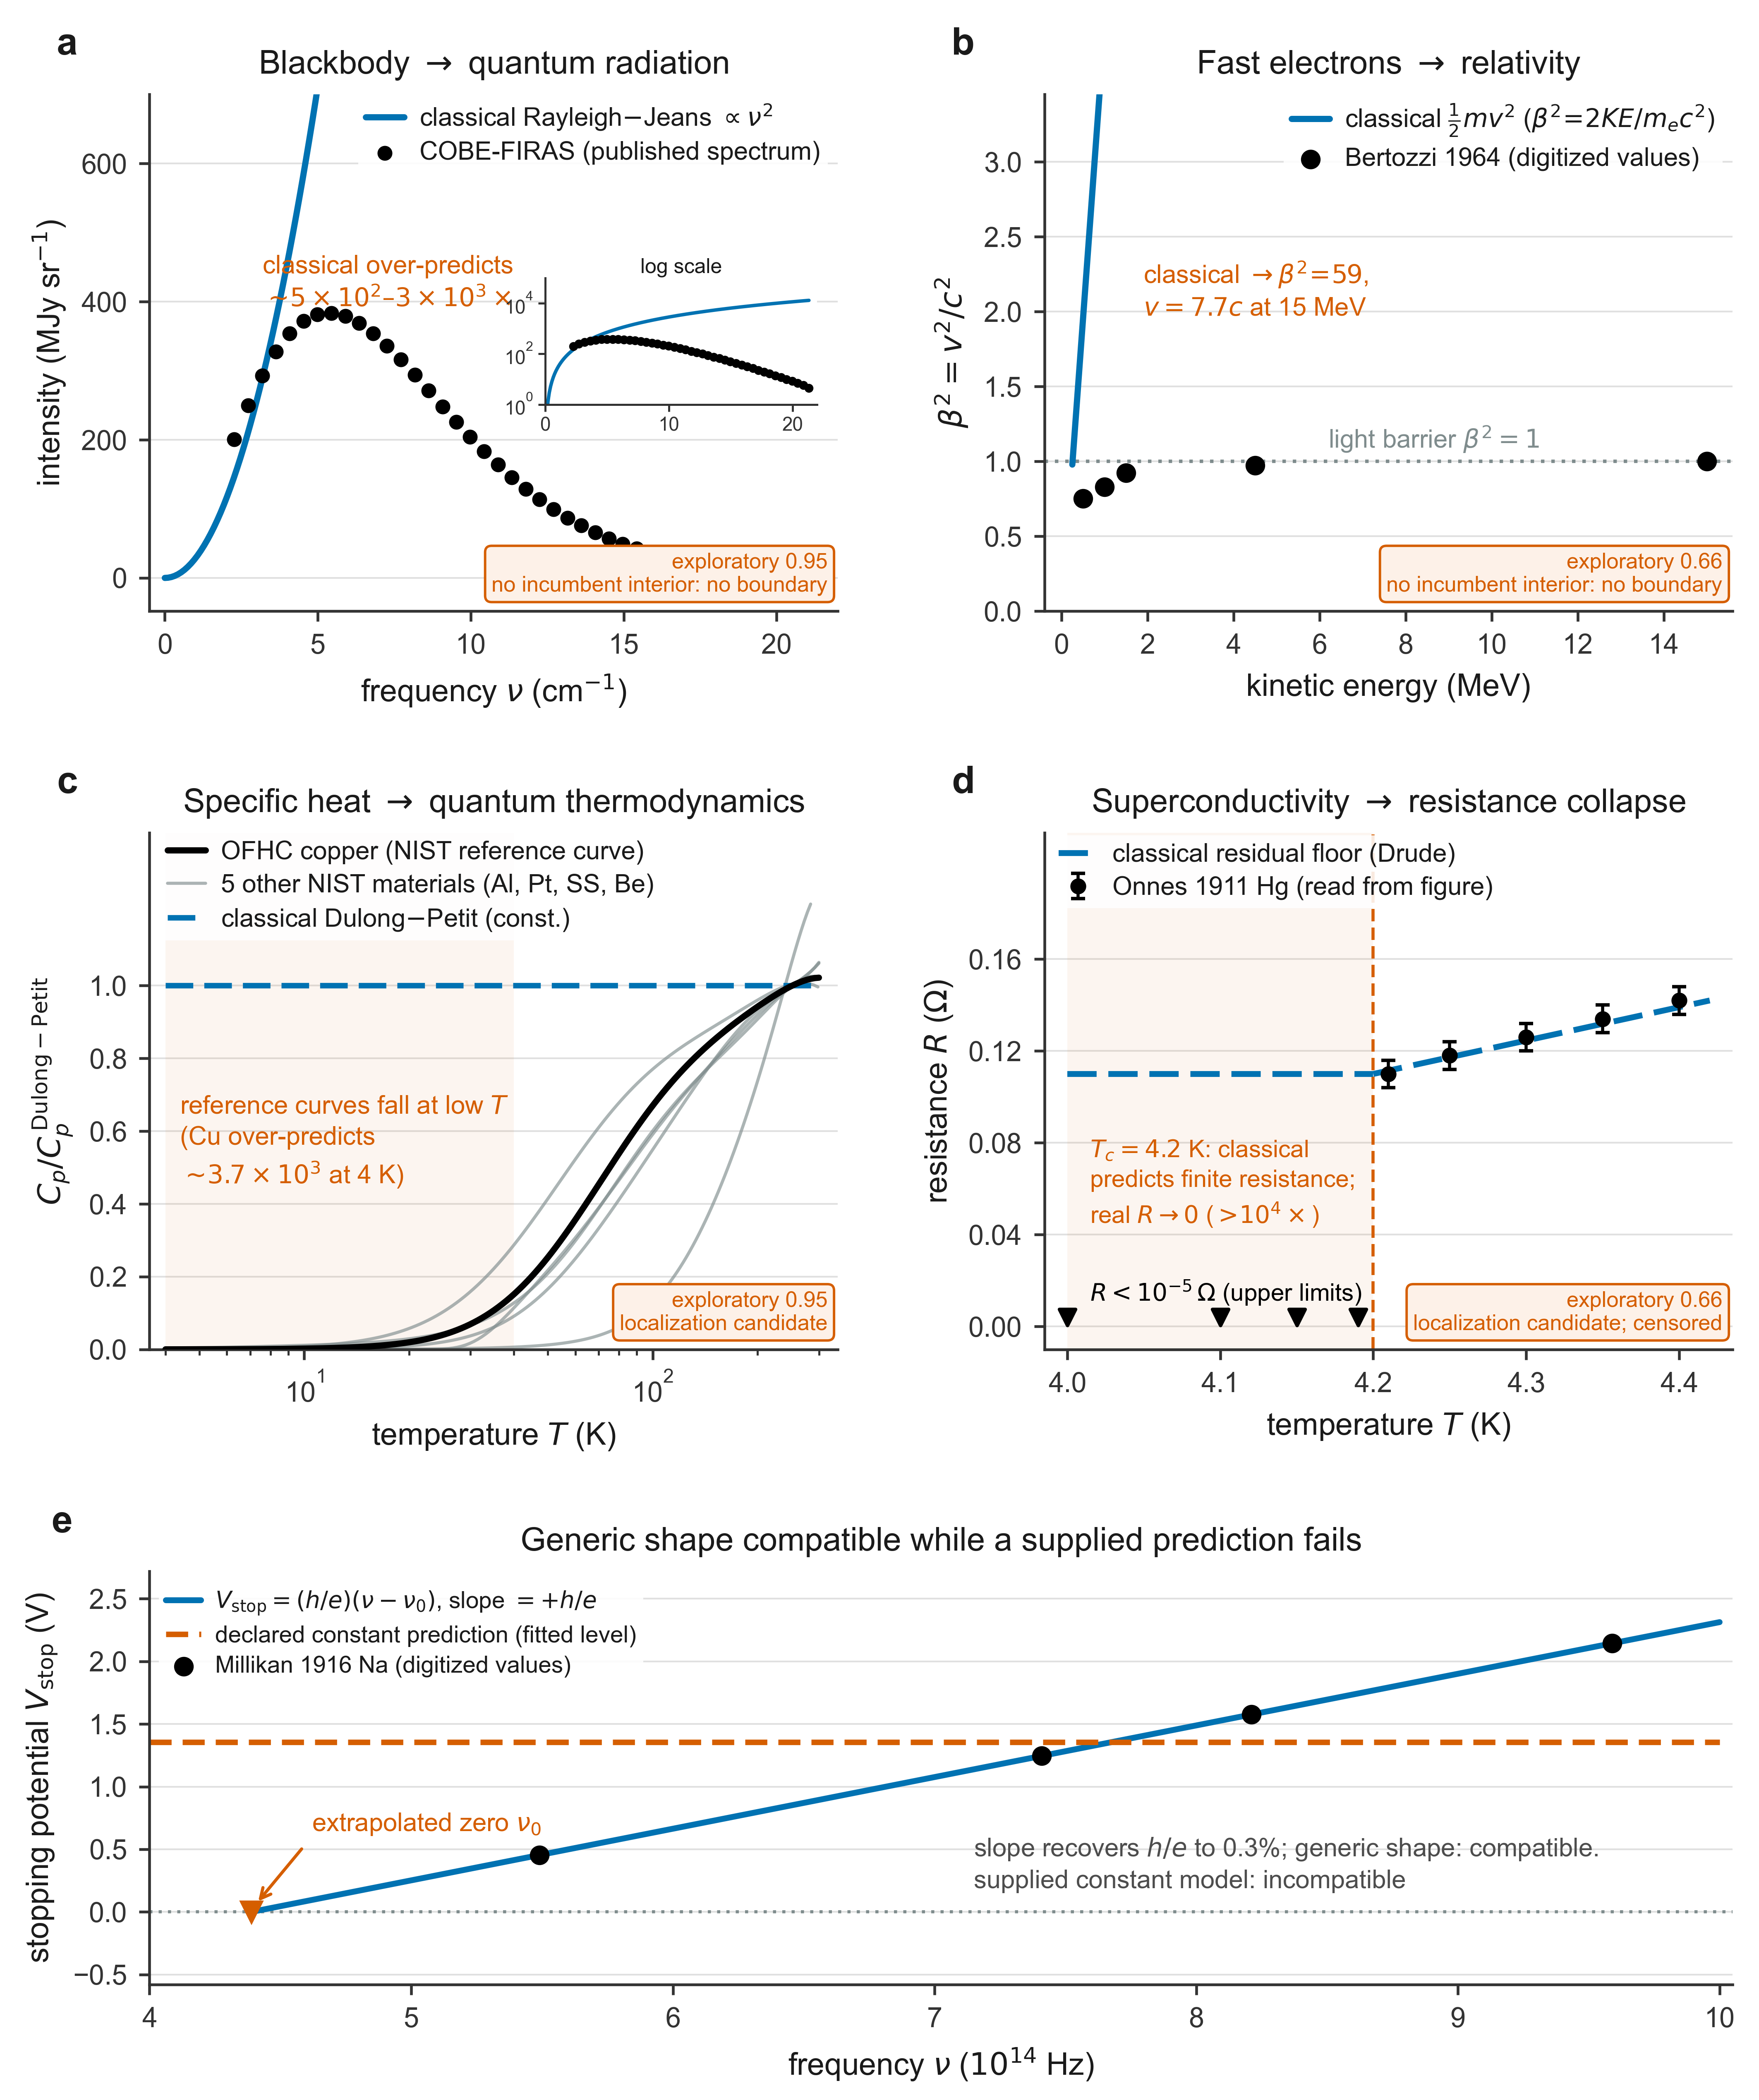
\includegraphics[width=\textwidth,keepaspectratio]{figures/figure_cases.png}
  \caption{\textbf{Historical measurements under the 1899 horizon. a--d}, Black
  points show published processed measurements, digitized historical values or
  evaluated reference curves as labelled; blue curves show incumbent predictions.
  Orange badges give screening percentiles. FIRAS and Bertozzi yield whole-range
  model rejection. Specific heat and Onnes contain an incumbent segment, allowing
  a candidate boundary to be marked by the shaded frontier. Tail probabilities
  and multiplicity calculations are reported in Supplementary Note~5.
  \textbf{e}, In Millikan's 1916 digitized values, stopping potential rises
  linearly with frequency as $V_{\mathrm{stop}} = (h/e)(\nu - \nu_{0})$. The
  slope recovers $h/e$ to 0.3\%, and the marker denotes the extrapolated zero
  crossing $\nu_{0}$. The generic shape score clears the line, whereas the
  theory-conditioned component rejects the classical prediction of
  frequency-independent energy (dashed line).}
  \label{fig:cases}
\end{figure}

In the 43-point COBE-FIRAS cosmic-microwave-background monopole
spectrum~\cite{fixsen1996firas}, a Rayleigh--Jeans law~\cite{rayleigh1900,jeans1905} proportional to $\nu^{2}$
over-predicts measured intensity above the peak by 475-fold to 3,000-fold across
fitting windows; the 20\% window gives a bootstrap interval of [1,500, 2,400]. At
$T = 2.725$~K, FIRAS samples $x = h\nu/kT$ from 1.2 to 11.3 rather than the pure
Rayleigh--Jeans regime $x \ll 1$, so the output is whole-range incompatibility
with the declared classical prediction rather than a located boundary.

Bertozzi's electron measurements\cite{bertozzi1964} report kinetic energy against
$\beta^{2} = v^{2}/c^{2}$. The classical law $\tfrac{1}{2}mv^{2}$ crosses
$\beta^{2} = 1$ near 0.26~MeV and reaches $\beta^{2} = 58.7$ at 15~MeV,
equivalent to $7.7c$, whereas the measurements approach $\beta^{2} = 1$. The
lowest point is already $0.87c$, placing the complete series outside a
non-relativistic interior, and EPOCH rejects the Newtonian energy--velocity
prediction over the sampled range.

The Dulong--Petit law~\cite{dulong1819} predicts temperature-independent molar heat capacity,
whereas the NIST cryogenic reference curves for six solids fall at low
temperature. Five materials contain a high-temperature plateau and support
candidate localization relative to the constant model; beryllium supports
whole-range incompatibility. Interior $R^{2}$ ranges from 0.965 to 0.998 and
departure ratios from 127 to 1,490, and for OFHC copper the classical
extrapolation over-predicts the 4~K reference value by roughly
$3.7\times10^{3}$. The reference-polynomial curves share one low-temperature
mechanism and are grouped accordingly.

Onnes's mercury resistance values~\cite{onnes1911}, digitized from $R(T)$ and
anchored by the reported resistance below $10^{-5}\,\Omega$, show a smooth
normal-state trend followed by a discontinuous drop. Relative to the declared smooth and residual-resistance models~\cite{drude1900}, EPOCH localizes a candidate boundary near
4.20~K, with figure-reading uncertainty and censored lower values carried into
the case-specific evidential status.

Millikan's 1916 photoelectric measurement shows why shape evidence and theory
evidence must be reported apart~\cite{millikan1916}. Stopping potential is linear
in frequency, $V_{\mathrm{stop}} = (h/e)(\nu - \nu_{0})$, with $R^{2} = 0.996$
and a slope that recovers $h/e$ to 0.3\% (Fig.~\ref{fig:cases}e), so the generic
dictionary accepts the shape without objection. The same four measurements
reject the classical prediction of frequency-independent photoelectron energy.
Their fitted intercept gives $\nu_{0} = 4.39\times10^{14}$~Hz, and because all
four frequencies lie above $\nu_{0}$ the output is whole-range model rejection
rather than localization of the emission threshold.

Three measured controls span two branches of physics and three and a half
centuries of measurement (Supplementary Fig.~1a--c). Independently measured
Solar-System orbits recover Kepler's exponent of 3/2~\cite{kepler1619} to four figures (1.500) and
score 0.02, the four Galilean moons give exponent 1.500 and score 0.00, and
Boyle's original 1662 pressure--volume table~\cite{boyle1662} gives exponent $-0.998$ and scores
0.38. All three fall below the 0.5 screening threshold.

\subsection{Advancing the horizon on the same measurements}

A calibrated mismatch is informative only if it tracks the declared model rather
than the data, so each dataset is scored twice on the same grid and under the
same error model: first under its old incumbent prediction, then under the
historically successful successor. The old horizon is rejected in all five cases
(bootstrap $p = 0.001$; Fig.~\ref{fig:calibration}a). The advanced horizon clears
FIRAS under Planck's law~\cite{planck1901} ($p = 1.000$), Bertozzi under relativistic kinetic
energy~\cite{einstein1905relativity} ($p = 0.089$), Onnes under a superconducting transition model
($p = 1.000$) and Millikan under the photoelectric relation~\cite{einstein1905photoelectric} ($p = 0.900$), with
mismatch statistics falling by factors from approximately $2.0\times10^{4}$ to
$7.3\times10^{10}$.

\begin{figure}[t]
  \centering
  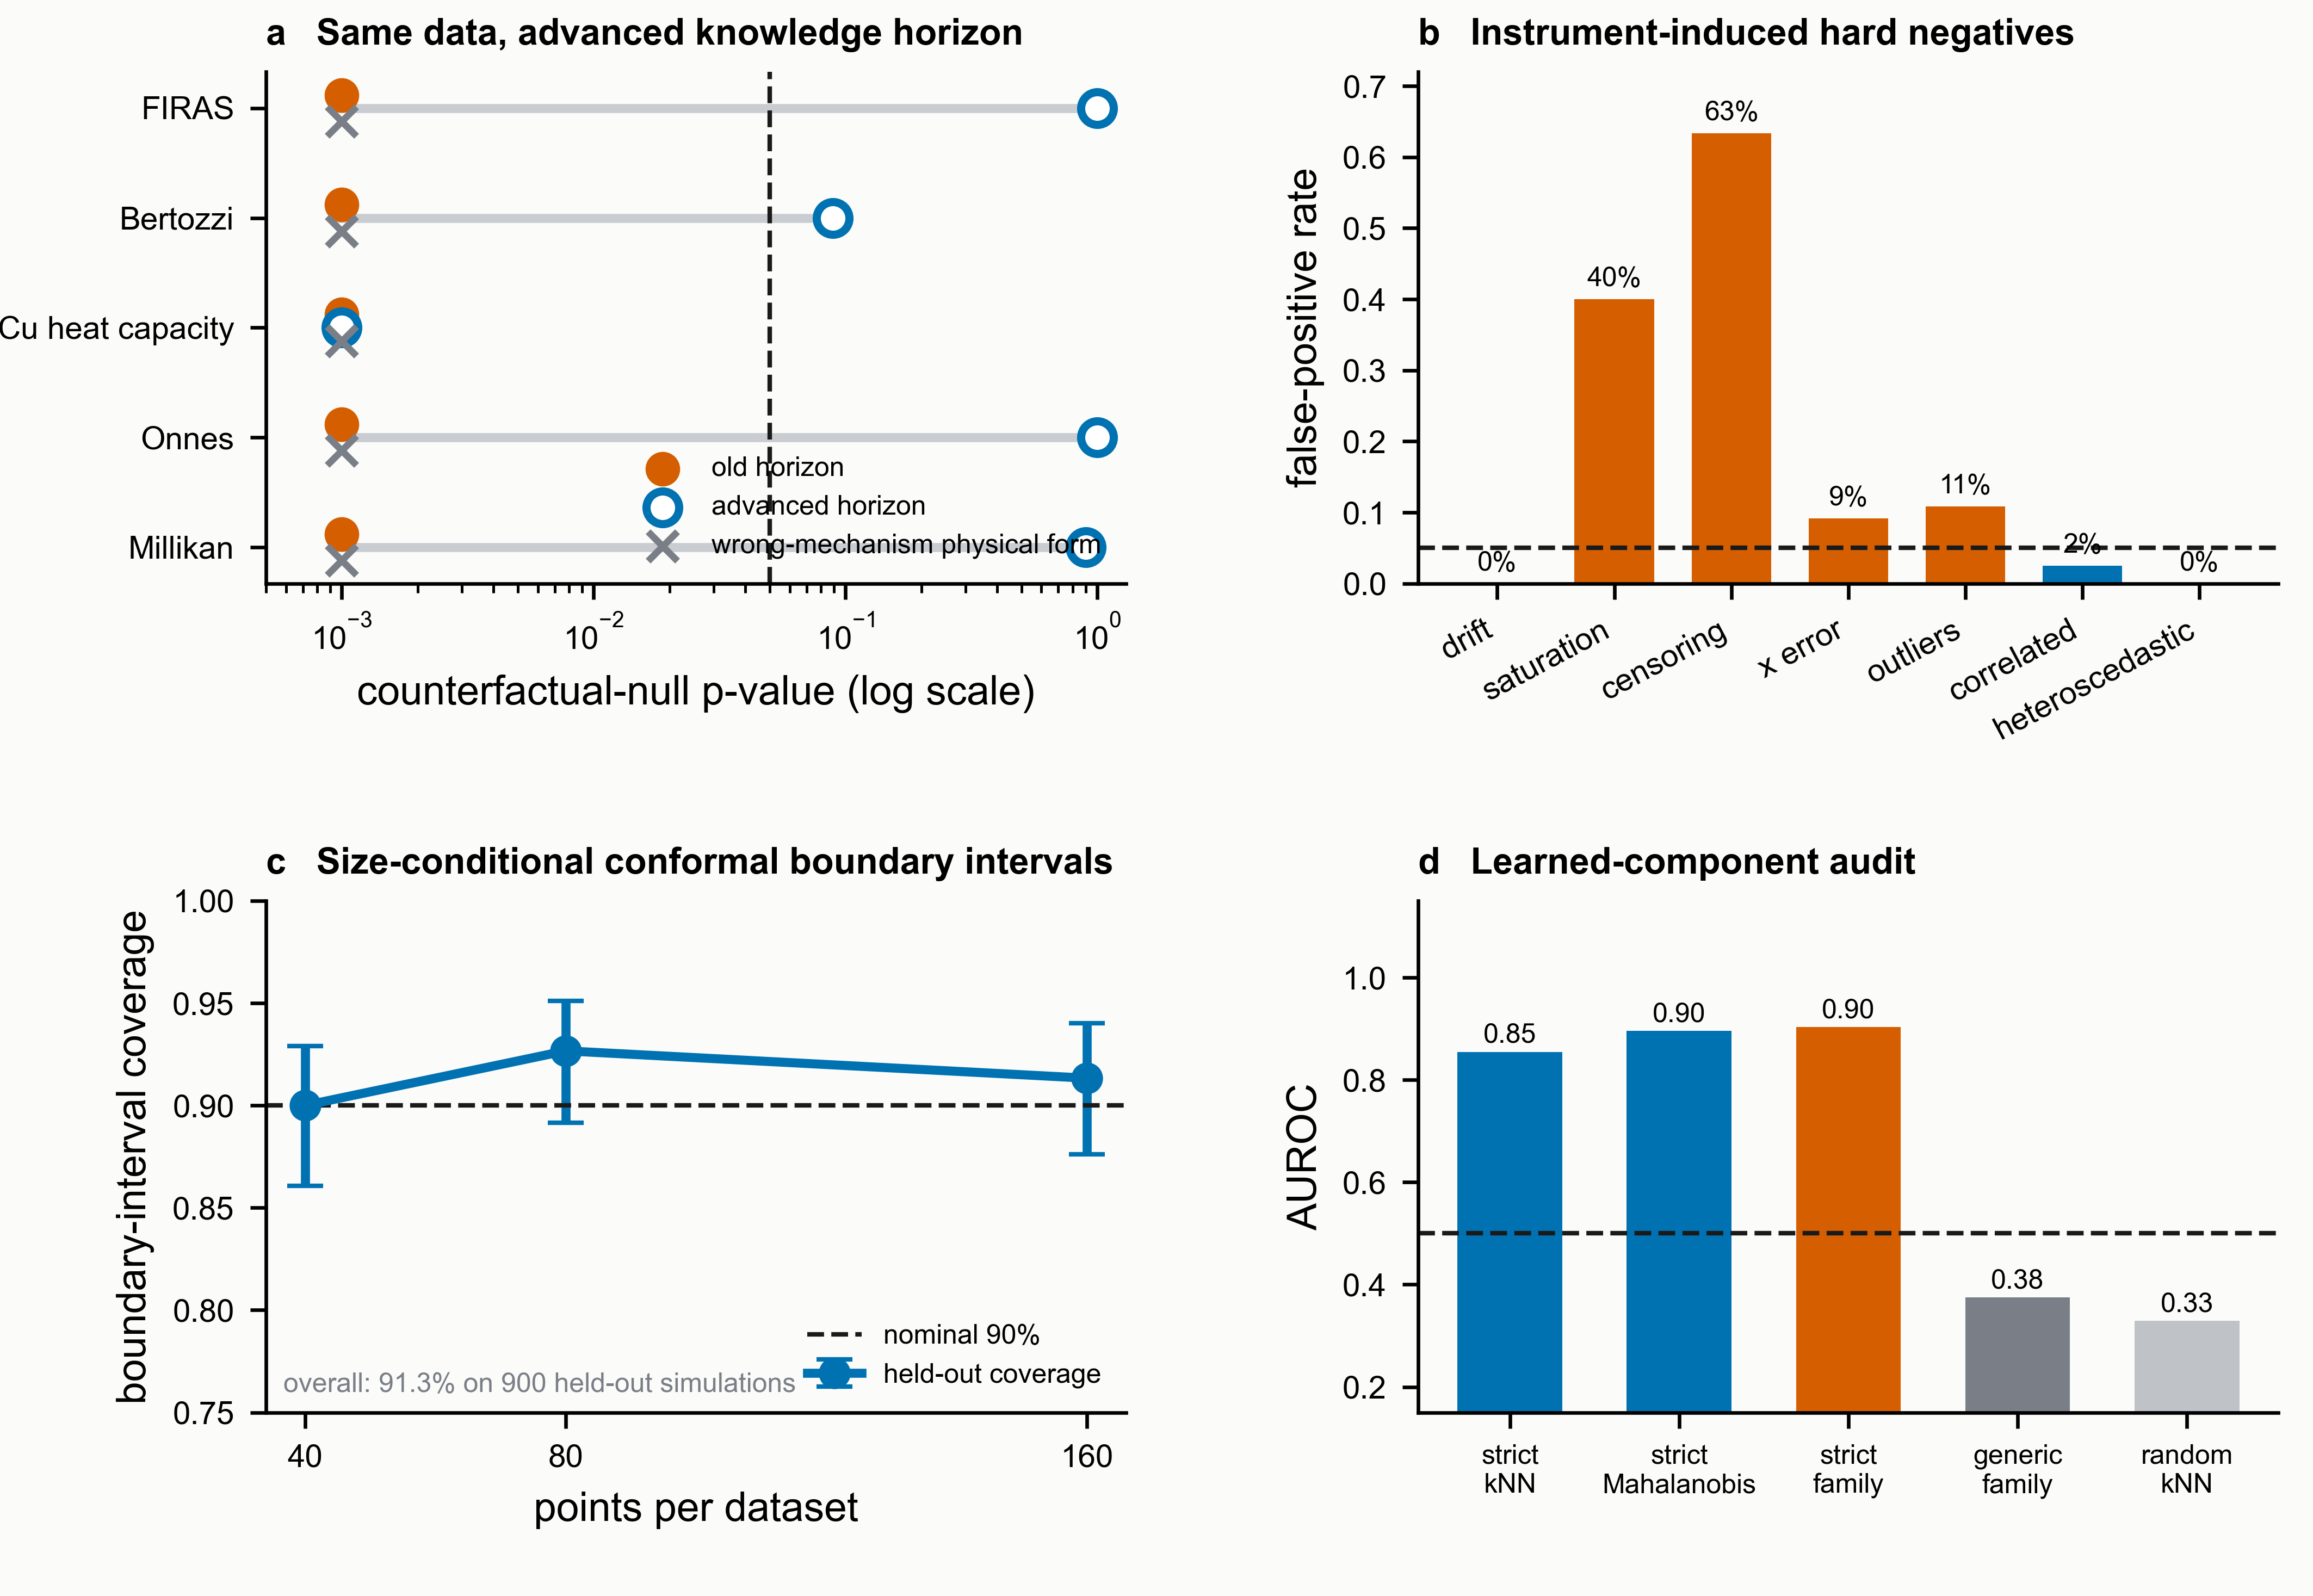
\includegraphics[width=\textwidth,keepaspectratio]{figures/figure_component_calibration.png}
  \caption{\textbf{Calibration and controls for the EPOCH components. a},
  Same-grid goodness-of-fit $p$-values under old and advanced horizons. Four of
  five advanced predictions clear at 5\%; five wrong-mechanism forms remain
  rejected. \textbf{b}, False-positive rates under simulated instrument effects,
  with the largest changes caused by saturation and censoring. \textbf{c},
  Held-out coverage of size-conditional 90\% split-conformal boundary intervals.
  \textbf{d}, Positive-only learned audit after source reconstruction. The
  zero-unit encoder reaches synthetic AUROC 0.854 by kNN and 0.895 by shrinkage
  Mahalanobis; family-grouped AUROC is 0.903 [0.729, 1.000], against 0.329 and
  0.288 for matched random features. Training uses 205 records from 40 pre-1900
  families and no breakdown examples. At the frozen family threshold it detects
  2/12 breakdown families while clearing all classical controls. The matched
  generic-function model reaches family AUROC 0.375 [0.167, 0.618] on the same
  evaluation families, a paired difference of 0.528 [0.264, 0.764]; across three
  paired seeds pre-1900 and generic AUROCs range over 0.889--0.910 and
  0.292--0.403.}
  \label{fig:calibration}
\end{figure}

Copper heat capacity is the exception and is sensitive to the error model. A
Debye-plus-electronic form~\cite{debye1912} reduces mismatch by $3.86\times10^{3}$ but remains
rejected under a 5\% reference-curve error floor ($p = 0.001$), clearing at
7.5\%. Across all five cases, low-dimensional wrong-shape families remain
rejected after Benjamini--Hochberg correction ($q \leq 0.0015$), as do
dimensionally coherent but mechanism-irrelevant physical forms (1,000 bootstrap
replicates; $p = q = 1/1001$). Four of the five score collapses are therefore
specific to the successful successor prediction rather than to any
better-fitting curve.

\subsection{Measured series at the same horizon}

Frozen components applied to sixteen unmodified NIST measurement series rank the
five post-1900 mechanism groups above the nine classical and metrological groups
with AUROC 0.62 [0.29, 0.89] for the learned score and 0.78 [0.38, 1.00] for the
four-form score (Fig.~\ref{fig:measured} and Supplementary Note~18). For each
series the column semantics, the 1899 incumbent and the mechanism group that
serves as the inferential unit are declared from its primary source before
scoring; neither component is retrained or recalibrated, measured series pass
through a rescale-only view function that adds no synthetic noise, and all 128
measurement-view scores are released.

\begin{figure}[t]
  \centering
  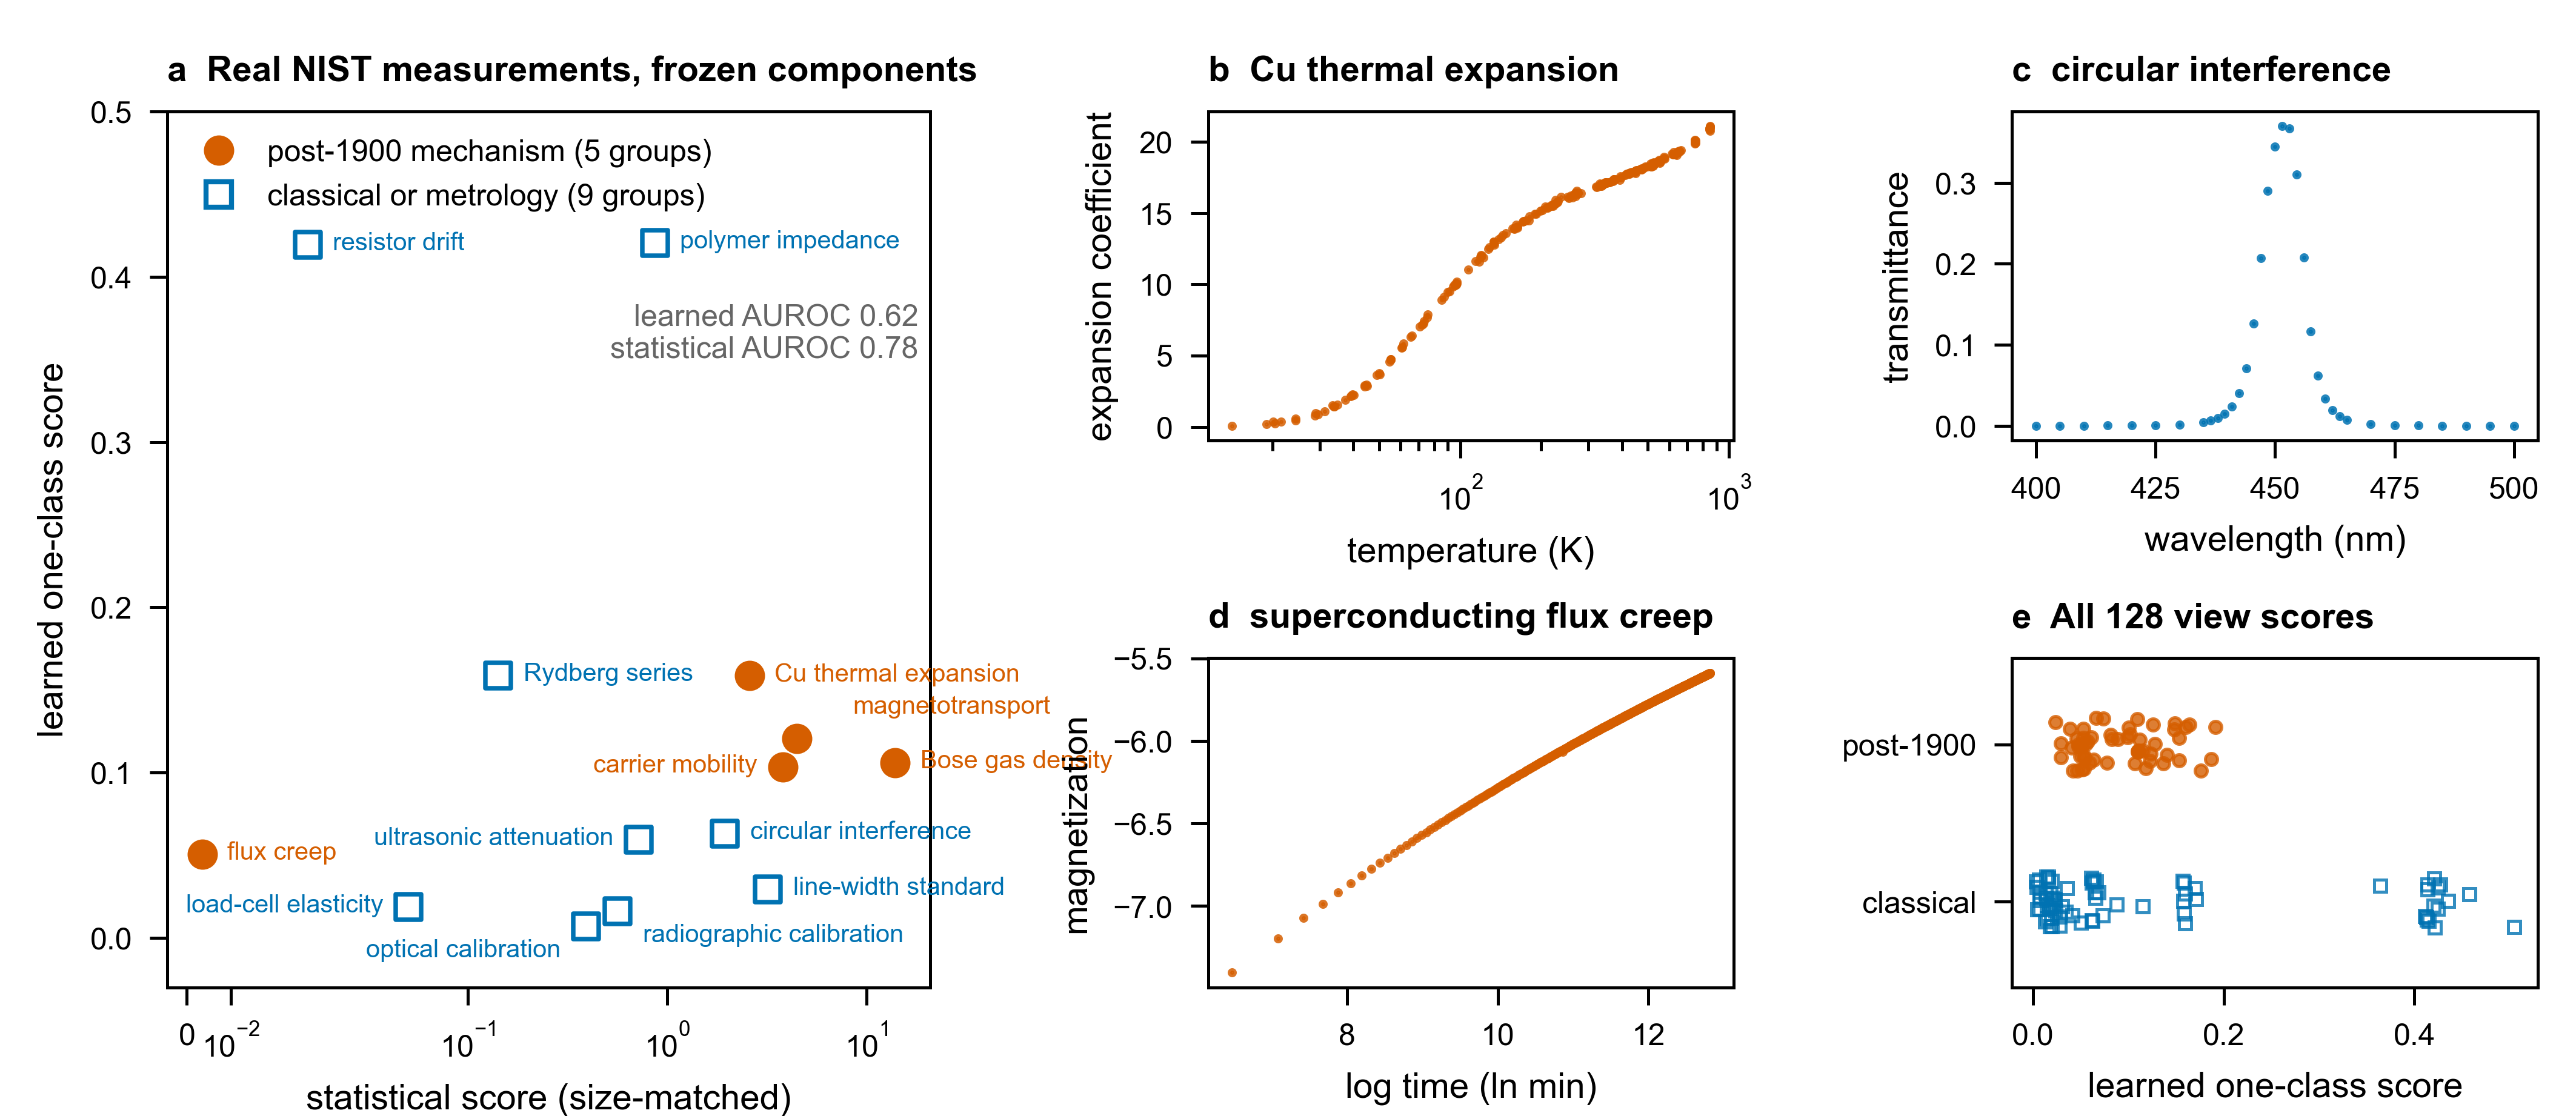
\includegraphics[width=\textwidth,keepaspectratio]{figures/figure_real_measurement_cases.png}
  \caption{\textbf{Frozen components on measured series. a}, Mechanism-group
  medians of the learned and four-form scores for sixteen NIST measurement series
  in fourteen groups, five outside the pre-1900 model set and nine classical or
  metrological. \textbf{b--d}, Three of the measured series: copper thermal
  expansion from 24~K to 852~K, circular-interference transmittance, and
  superconducting magnetization relaxation against log time. \textbf{e}, Every
  individual measurement-view score behind the medians in \textbf{a}. The
  released quantity is the continuous component output.}
  \label{fig:measured}
\end{figure}

Copper thermal expansion measured from 24~K to 852~K takes the highest post-1900
learned score, its coefficient falling towards zero below the Debye temperature
in a way classical equipartition of lattice modes cannot produce~\cite{einstein1907solid}, and the
density profile of a cold Bose gas~\cite{bose1924,andersonbec1995} takes the highest four-form score. A sulfur
Rydberg series~\cite{rydberg1890}, whose inverse-square form was available empirically in 1888,
belongs to the classical class yet ranks above four of the five post-1900
groups.

Two series bracket what the components read from measured data.
Circular-interference transmittance rises to a sharp resonance at 451~nm, the
most unusual shape in the collection, yet scores low on both components, so
morphological novelty by itself moves neither coordinate. Superconducting
magnetization relaxation, which no pre-1900 theory accounts for, is close to
logarithmic in time and takes the lowest four-form score of any series. Across
the whole collection the two highest learned scores belong to a five-year
standard-resistor record and a 23-point polymer-impedance curve: on measured data
the leading axis of variation is the observation process rather than the period
of the underlying physics. Fourteen mechanism groups set the width of both
intervals.

\subsection{Calibration, thresholds and the observation process}

On the 36-dataset fair suite the statistical detector reaches AUROC
0.80 [0.64, 0.94], against 0.58 for Gaussian-process discrepancy~\cite{rasmussen2006} and 0.77 for
split-conformal prediction (Supplementary Fig.~1d,f). Withholding the classical
law, or both the law and the interior regime, leaves AUROC at 1.00 and 0.97, so
the result does not depend on supplying the answer.

Calibrating the data-anchored score separately at $n = 5$, 9, 43 and 120 over 12
departure and 12 classical families fixes the operating point. At $n = 120$, TPR
is 0.271 [0.073, 0.500] at the frozen 5\% quantile and 0 at the 1\% quantile,
with a realized false-positive rate of 0/96 at both. Sensitivity is 1.0 for
smooth roll-off and discontinuous-drop simulations and zero for seven families,
so this operating point buys specificity at a known cost in power.

Altering the observation process while holding the underlying classical relation
fixed shows where that specificity fails. At the strongest simulated levels a
detector calibrated to 5\% reports false-positive rates of 0\% for calibration
drift, 40\% for sensor saturation, 63\% for censoring, 9\% for x-axis error,
11\% for outliers, 2.5\% for correlated noise and 0\% for heteroscedasticity
(Fig.~\ref{fig:calibration}b). The output schema therefore carries a
measurement-process branch, with saturation and censoring tested explicitly for
plateau and threshold cases.

Boundary estimates need the same treatment. Ordinary measurement bootstrap
intervals cover only 53.9\% of true onsets at a nominal 90\% level, and 8.5\% for
steps; size-conditional split-conformal radii calibrated on 899 independent
simulations raise held-out coverage to 91.3\% [89.3\%, 93.0\%] across 900
simulations, with family-wise coverage from 87.8\% for smooth turnovers to
94.4\% for kinks (Fig.~\ref{fig:calibration}c). The reported boundary is
therefore an interval rather than a single estimated onset.

Simulations extend the evaluation into incumbent regimes absent from the FIRAS
and Bertozzi measurements. Blackbody radiation spanning $x = h\nu/kT$ from well
below to well above unity contains a Rayleigh--Jeans interior with
$R^{2} = 0.99$ followed by a departure with conformal score 468 and ratio 192;
relativistic kinetic energy yields a localized boundary at $0.86c$, and simulated
photoelectric voltage localizes the frequency threshold.

\section{Discussion}

We introduced a test of a declared knowledge horizon and applied it at 1899.
Trained only on source-audited pre-1900 relations, with no later formula and no
breakdown template in its optimization, a 20.9-million-parameter encoder ranks 55
twentieth-century formula families above nine held-out pre-1900 groups at AUROC
0.925, against 0.649 for the same architecture before optimization; regenerating
those controls under the later benchmark's sampling and noise process leaves
0.857, and an independently frozen four-form scorer reaches 0.888 on the same
comparison.

A mismatch is interpretable only when it is tied to a named incumbent model.
Scoring each historical dataset twice on the same grid and under the same error
model, four of five old-horizon discrepancies disappear once the successful
successor prediction is admitted, while wrong-shape and dimensionally coherent
wrong-mechanism alternatives stay rejected after multiplicity correction. Copper
heat capacity is the exception, and its behaviour is informative: the advanced
model clears only when the reference-curve error floor is relaxed from 5\% to
7.5\%, so the observation model belongs to the knowledge horizon rather than to
the nuisance parameters. For a closed-form theory, advancing the horizon amounts
to replacing the admitted prediction and recalibrating its reference
distribution, and simulator-based references give the corresponding construction
where no closed form exists.

Shape novelty and predictive failure are not the same quantity. Later affine,
power and exponential laws often stay close to the generic dictionary, whereas
threshold, piecewise, nonmonotone and oscillatory relations separate strongly;
conversely a physically decisive discrepancy can keep an entirely ordinary shape,
as Millikan's stopping potential and the Pound--Rebka redshift both do. The
measured series make the point from both directions. A classical
circular-interference resonance, the most unusual morphology in that collection,
scores low on both components, while superconducting flux creep~\cite{anderson1964fluxcreep}, which no
pre-1900 theory accounts for, is close to logarithmic in time and sits at the
bottom of the four-form ranking. Keeping the component scores separate rather
than averaging them is what preserves this distinction.

Several limitations bound what these results establish. Although the 1899
experiment is internally controlled, its negative class is small: nine held-out
pre-1900 groups carry the primary learned comparison and set the width of its
interval, and the generator-matched analysis was registered after the primary
scores were opened. The native generator-gated comparison gives AUROC 0.536, so
the sampling process remains an active component of the native contrast and the
matched value of 0.857 is the estimate that controls for it. On measured series
the ranking falls to 0.62 for the learned component and 0.78 for the four-form
component, with intervals that span chance, and the two highest learned scores in
that collection belong to a standard-resistor record and a polymer-impedance
curve rather than to any physical departure --- the same sensitivity that
saturation and censoring expose in the simulated instrument tests.

EPOCH draws on neural extrapolation~\cite{wang2023discovery,xu2021extrapolate},
split-conformal prediction, Bayesian model discrepancy and change-point
detection~\cite{angelopoulos2023conformal,page1954cusum,kennedy2001bayesian}, and
shares machinery with model-independent searches in particle
physics\cite{dagnolo2019newphysics} and with machine rediscovery of natural
laws~\cite{guimera2020bayesian,udrescu2020feynman,schmidt2009distilling}. What
differs is the target of inference: EPOCH tests the predictive domain of a
declared model before asking symbolic regression or theory construction for a
replacement. Once a calibrated mismatch exists, that search can proceed under a
parsimony prior~\cite{he2026searchfree}, as the Bayesian machine scientist and AI Feynman do in
recovering Planck-type expressions from
blackbody-type data~\cite{guimera2020bayesian,udrescu2020feynman}, and physical
interpretation then supplies the mechanism behind the fitted form.

Large libraries of measured relations can be ranked against a frozen horizon, and
selected cases rerun with explicit measurement errors and incumbent predictions
to obtain a model test and, where an incumbent regime is sampled, a boundary
interval. Moving the interface to another period requires only a different dated
corpus, admitted prediction and calibration set. The decisive next experiment
freezes the full decision path in advance and runs it against
mechanism-independent measurements whose instrument models have been audited, so
that the observation process is known rather than assumed.

\section{Methods}

\subsection{Declaring a test}

An EPOCH test is the tuple
$\mathcal{T}=(\mathcal{M},\Theta,P_\varepsilon,I,A,S,\alpha)$, in which
$\mathcal{M}$ is the admissible model set, $\Theta$ the fitted parameters,
$P_\varepsilon$ the observation and censoring model, $I$ the fitting data, $A$
the complete adaptive procedure, $S$ the discrepancy statistic and $\alpha$ the
error rate. Because direction choice, window search, model selection and
parameter fitting all belong to $A$, each of them is rerun inside every
calibration and null replicate rather than being fixed once on the test data.
Confirmatory tests use the finite-sample upper-tail probability
$p=(1+\#\{S_i\geq S_*\})/(n_{\mathrm{cal}}+1)$ with ties counted conservatively,
and dataset scans report Benjamini--Hochberg adjusted
$q$-values~\cite{benjamini1995fdr}. The primary endpoint is the true-positive rate
at a threshold targeted to 5\% false positives on independent calibration, with
the 1\% threshold secondary; the 0.5 percentile used in the historical screen is
a screening threshold and not a rejection criterion. Exchangeability is defined
at the level of the source-law family or mechanism family, so the guarantee that
follows applies to the declared exchangeable generator rather than to an
arbitrary frontier.

\subsection{Generic dictionary and the interior--frontier split}

The data-anchored component draws on a fixed parsimonious vocabulary of power,
exponential, linear and constant forms. An eight-form ablation adding quadratic,
cubic, square-root and logarithmic terms was tested and discarded, because the
four-form version extrapolates better on validation data. Given a point cloud, a
fixed rule takes the candidate interior to be the contiguous regime in which one
admitted form fits with high internal $R^{2}$, and the frontier to be the
complementary region; the search runs from both ends and fit quality decides
whether the low- or the high-value direction is retained. Split-conformal nonconformity~\cite{vovk2005} is then computed from interior residual quantiles, and the
extrapolation-residual ratio compares the median log-residual at the frontier
with its interior value. Each form is fitted from several initializations, and
both denominators carry a one-percent relative floor so that a near-perfect
interior fit cannot produce an unbounded ratio. A capped variant, which averages
rescaled components clipped at 3, is retained for comparison with earlier
results. Relations with fewer than 20 points are calibrated against size-matched
simulations.

\subsection{Large-scale pre-1900 representation}

The scaling experiment uses a 20,908,547-parameter dual encoder trained without
any anomaly supervision. Its query branch is a permutation-invariant six-block
Set Transformer\cite{lee2019settransformer} of width 384 with eight heads, four
pooling tokens and a 256-dimensional normalized output, and during positive-only
pretraining it is aligned to a formula-structure teacher built from four
edge-aware graph updates and two graph-local attention layers, one of whose
update networks is a 96-channel eight-basis RBF-KAN module~\cite{liu2025kan}. At
query time the encoder receives a median/IQR-normalized unordered $(x,y)$ cloud
and nothing else: no equation, graph, units, date, law name, post-cutoff label or
deformation example.

Training draws on 880,896 normal-law clouds derived from 3,441 audited pre-1900
formula reductions, grouped into 91 contrastive identities that span 64
historical-family tags, with held-out calibration and internal sets of 11,648 and
62,336 clouds from 91 and 487 formulas. Reducing these to scientific groups
leaves nine historical-family groups, which form the internal control class for
every AUROC reported here. The model trains for 30 epochs at batch size 1,024
under a checkpoint rule fixed before any temporal evaluation. Its one-class score
averages four calibrated ranks --- top-eight cosine distance to graph-formula
embeddings, top-eight distance to identity centroids, top-eight distance to
point-formula prototypes, and shrinkage-Mahalanobis distance~\cite{mahalanobis1936,ledoit2004} to those prototypes
--- each transformed by its own pre-1900 calibration empirical CDF. Clouds are
reduced by median to formulas and then to source-law families or frozen relation
groups, and family- and group-level AUROCs use 2,000 grouped-bootstrap
replicates. An architecture-matched, same-seed checkpoint that has received no
optimization passes through the identical pipeline. Code, configuration, score
construction, seed and checkpoint rule were timestamp-frozen before the first
temporal score was computed.

For the generator-matched analysis, all nine internal control families were
regenerated with the temporal benchmark's point count, x-jitter, repeat count,
noise range and heteroscedastic profile, while the checkpoint, reference
memories, calibration CDF, score and aggregation were left unchanged; the same
analysis was then repeated with the zero-optimization checkpoint. A separate
96,064-cloud generator-gated set and the cumulative pre-1950 pilot are reported
in Supplementary Note~16.

\subsection{Compact encoder and its controls}

The compact set transformer has width 128 and three induced-set-attention blocks,
and trains for 1,000 steps on two independently subsampled and rescaled views of
205 source-audited classical point clouds drawn from 40 families. Families are
sampled without replacement so that repeated laws cannot become false contrastive
negatives, and an auxiliary head predicts functional signatures. No breakdown,
saturation, step, kink, splice or crossover example enters this optimization.
Matched models are trained with SI dimensions and with zeroed dimension metadata,
and the zero-unit model is primary for the synthetic benchmark. Frozen one-class
kNN and shrinkage-Mahalanobis scores are compared against a matched random
encoder. Cross-conformal calibration removes each training family in full,
reduces the eight measurement views within a record and then reduces records to
one median per family; the higher-order 95th-percentile statistic over the 40
leave-family-out family scores is frozen before evaluation, and hash-linked
training and evaluation files enforce checkpoint and data identity.

Three controls bound what this representation has learned. A second zero-unit
encoder shares architecture, seed, batch size, augmentation, auxiliary objective
and 1,000-step schedule but is trained on 205 point clouds from globally valid
smooth expressions in 40 pseudo-families, matched to the historical set in record
count, family-size profile and the histogram of eight-bit functional signatures.
Both encoders are retrained from scratch under three paired initialization and
augmentation seeds while the evaluation-view seed and the 24 mechanism families
stay fixed, and we report the observed range and sample standard deviation across
those runs without altering the canonical checkpoints. Finally, each of 46
held-out point clouds is paired with saturation, step, kink, splice, roll-off and
crossover deformations that retain its archived input and output SI vectors;
scores reduce to one clean and six deformation values within each of seven
source-law families, the AUROC difference is bootstrapped by family, and each
checkpoint is read against its own higher-order 95th-percentile threshold.
Thirty-four of those records carry at least one nonzero dimensional exponent.

Routing for the learned component is fixed in advance. Point clouds with at least
20 observations receive a learned score, near-constant responses route instead to
a theory-conditioned constant-or-noise model, and formula and deformation
families are the resampling units throughout. Where a deformation-supervised
probe is quoted for comparison, it carries explicit anomaly-shape priors, whereas
the positive-only encoders reported as primary see normal pre-1900 relations
alone.

\subsection{Frozen post-1900 formula transfer}

The transfer registry contains 55 source-law families first valid between 1901
and 1996, each carrying a primary historical citation and 45 of them a DOI, spanning thermionic emission~\cite{richardson1901} through discrete atomic excitation~\cite{franck1914}, parity violation~\cite{wu1957}, absence of diffusion in disordered lattices~\cite{anderson1958}, the local-hidden-variable bound and its experimental test~\cite{bell1964,aspect1982} and the first gravitational-wave detection~\cite{abbott2016}. Every
law is represented by a disclosed one-dimensional nondimensional reduction over a
fixed support, realized eight times at 120 points with varying nuisance
parameters, sampling and 0.5--2.5\% noise, giving 440 records across 55
inferential units. Special reductions, among them the BCS interpolation~\cite{bardeen1957}, the
two-flavour neutrino survival curve~\cite{maki1962} and the ideal quantum-Hall staircase~\cite{klitzing1980}, are
marked as such in the registry, and offline checks cover family and seed
uniqueness, citation-year consistency, finite nonconstant curves, point ordering,
file hashes and separation from the pre-1900 archive.

No training or calibration takes place during transfer. The checkpoint and the
pre-1900 data hash must match those of the cross-family audit before scoring
begins. The learned score is reduced by median over measurement views, records
and families and read against the pre-existing higher-order $q_{95}$ statistic
from the 40 leave-family-out calibration families, while the statistical score
reruns the full four-form selection and extrapolation procedure against the
existing $n = 120$ thresholds. Eleven cited pre-1900 families serve as controls,
AUROC intervals resample families, and twelve of the post-1900 laws deliberately
overlap the declared affine, power or exponential forms. Per-family conformal
$p$-values and component union and intersection rates are reported as secondary
diagnostics.

\subsection{Historical measurements and horizon-specificity controls}

We analyse the published COBE-FIRAS monopole spectrum with its pointwise errors,
five Bertozzi values digitized from the 1964 report, NIST specific-heat reference
polynomials for six materials, Onnes resistance values including upper limits,
Millikan sodium stopping potentials and Solar-System orbital constants. Each case
is serialized as a test object recording input status, model set, fitted
parameters, observation model, fit subset, adaptive procedure, decision rule,
output and provenance. Old- and advanced-horizon counterfactual nulls are
evaluated on the same $x$-grid, and explicit error floors stand in for
unavailable covariance and for digitization uncertainty and are varied in
sensitivity analysis.

To establish that a collapse in mismatch is specific to the successful successor,
wrong-shape and dimensionally coherent wrong-mechanism forms are refitted on the
same case grids and observation models with 1,000 parametric-bootstrap
replicates. The physical controls substitute fermionic occupation for photon
statistics, a proton for the electron rest-energy scale, an Einstein oscillator~\cite{einstein1907solid}
for Debye acoustic modes~\cite{debye1912}, Arrhenius transport for the superconducting transition,
and Compton recoil for the photoelectric slope; dimensional ratios and parameter
units are retained in the machine-readable output.

\subsection{Measured series}

Sixteen series are taken unmodified from the NIST Dataplot and Statistical
Reference Dataset collections and bound to their SHA-256 hashes. A registry
declares, for each series, the numeric block, the abscissa and response columns,
the 1899 incumbent, the mechanism group and the horizon class before any score is
computed. Where a file header and its stored block disagree on column order, the
order is resolved against certified values, and a file that is a subset or
decimation of another series shares that series' mechanism group rather than
forming a second unit. Series are sorted by abscissa and thinned uniformly to at
most 2,000 points. The learned component applies the declared near-constant
routing rule and a rescale-only view function that adds no synthetic noise to a
measurement, with the reference bank rebuilt from the frozen pre-1900 training
split; the statistical component reruns the complete four-form direction, window,
model-selection and scoring procedure on eight subsamples drawn at the largest
frozen calibration size each series supports. Scores reduce by median within a
series and then within a mechanism group, and the grouped AUROC resamples
mechanism groups.

\subsection{Synthetic suites, baselines and localization}

The held-out evaluation comprises 180 labelled datasets and the fair baseline
suite 36, on which split-conformal prediction, the extrapolation-residual ratio,
Gaussian-process discrepancy~\cite{rasmussen2006}, CUSUM~\cite{page1954cusum} and RESET~\cite{ramsey1969} are compared. The mechanism-level
benchmark contains 12 classical and 12 breakdown families with eight realizations
each; its 5\% and 1\% thresholds come from 785 valid size-matched calibration
simulations, and uncertainty is resampled by mechanism family rather than
treating noise realizations as independent phenomena. The learned checkpoint
audit uses 192 datasets over the same 24 families. Instrument tests apply
calibration drift, sensor saturation, censoring, x-axis error, outliers,
correlated noise and heteroscedasticity to classical synthetic relations while
leaving the underlying law intact, and boundary intervals are obtained by
split-conformal calibration of the normalized localization error separately at
$n = 40$, 80 and 160.

\subsection{Real-measurement inventory}

Forty-four files were downloaded from the NIST Dataplot and Statistical Reference
Dataset collections and their SHA-256 hashes frozen. The inventory holds 20
instrument controls, 11 classical controls, six modern-known controls and seven
horizon cases. A dataset is promoted into the evaluation registry only once its
column semantics, incumbent prediction, measurement model, provenance and
mechanism-level grouping have been audited.

\section{Data availability}

The public COBE-FIRAS, Solar-System, Bertozzi, NIST, Millikan and Kamerlingh
Onnes inputs are identified in the Supplementary Information. The data package
contains source URLs and hashes; the 55-family formula registry and 440 generated
point clouds; the 11-family development registry and 88 generated records; the
pre-1900 training, calibration and evaluation manifests; and every numerical
result used in the figures. The project repository is available at
\url{https://github.com/ChenxiHeCam/Epistemic-probe-of-Classical-Horizons}, and
the archive for this release at \url{https://doi.org/10.5281/zenodo.22742368};
\url{https://doi.org/10.5281/zenodo.22138620} resolves to the most recent
version.

\section{Code availability}

Code is available at
\url{https://github.com/ChenxiHeCam/Epistemic-probe-of-Classical-Horizons}. The
repository contains corpus audits, point-cloud generators, frozen evaluators,
statistical calibration and robustness experiments, model definitions, training
configurations, figure scripts and the evidence-manifest validator. Checkpoint
and data hashes are verified before evaluation, and the release archived at
\url{https://doi.org/10.5281/zenodo.22742368} is the version used for every
number reported here.


\section{Acknowledgements}

We thank NASA LAMBDA, the NIST Cryogenic Material Properties database and the
KNAW digital archive for public data access. This research received no specific
grant from any funding agency in the public, commercial, or not-for-profit
sectors.

\section{Author contributions}

C.H. conceived the framework, designed and built EPOCH, ran the experiments, and
wrote the manuscript. J.C. contributed to the benchmark construction, case-study
analysis, and manuscript revision. Both authors reviewed and approved the final
manuscript.

\section{Competing interests}

The authors declare no competing interests.

\textbf{Correspondence and requests for materials} should be addressed to C.H.
(ch2067@cam.ac.uk).

\clearpage

\bibliographystyle{unsrtnat}
\bibliography{refs}

\end{document}
